\section*{Задание 1. Сжатие изображений с помощью SVD}

В качестве исходного изображения использована картинка из набора по предмету, переведённая в оттенки серого и представлена в виде матрицы интенсивностей \(A\in\mathbb{R}^{m\times n}\).

Было выполнено SVD-разложение \(A = U\,\Sigma\,V^\top\), после чего построены укороченные аппроксимации \(A_k = U_{[:,1:k]}\,\Sigma_{1:k,1:k}\,V_{[1:k,:]}\) для ряда значений \(k\). Ниже приведены исходное изображение и сетка реконструкций для девяти значений \(k\), а также графики ошибки восстановления (MSE) и относительного объёма хранения.

Численно степень сжатия оценивалась как
\[ \text{ratio}(k) = \frac{m k + k + k n}{m n}, \]
где числитель — количество значений для хранения укороченного разложения \(U_k,\Sigma_k,V_k\). Для представленных значений \(k\) график на рисунке~\ref{fig:svd-metrics} показывает компромисс между качеством (MSE) и объёмом хранения.

\begin{figure}[h!]
  \centering
  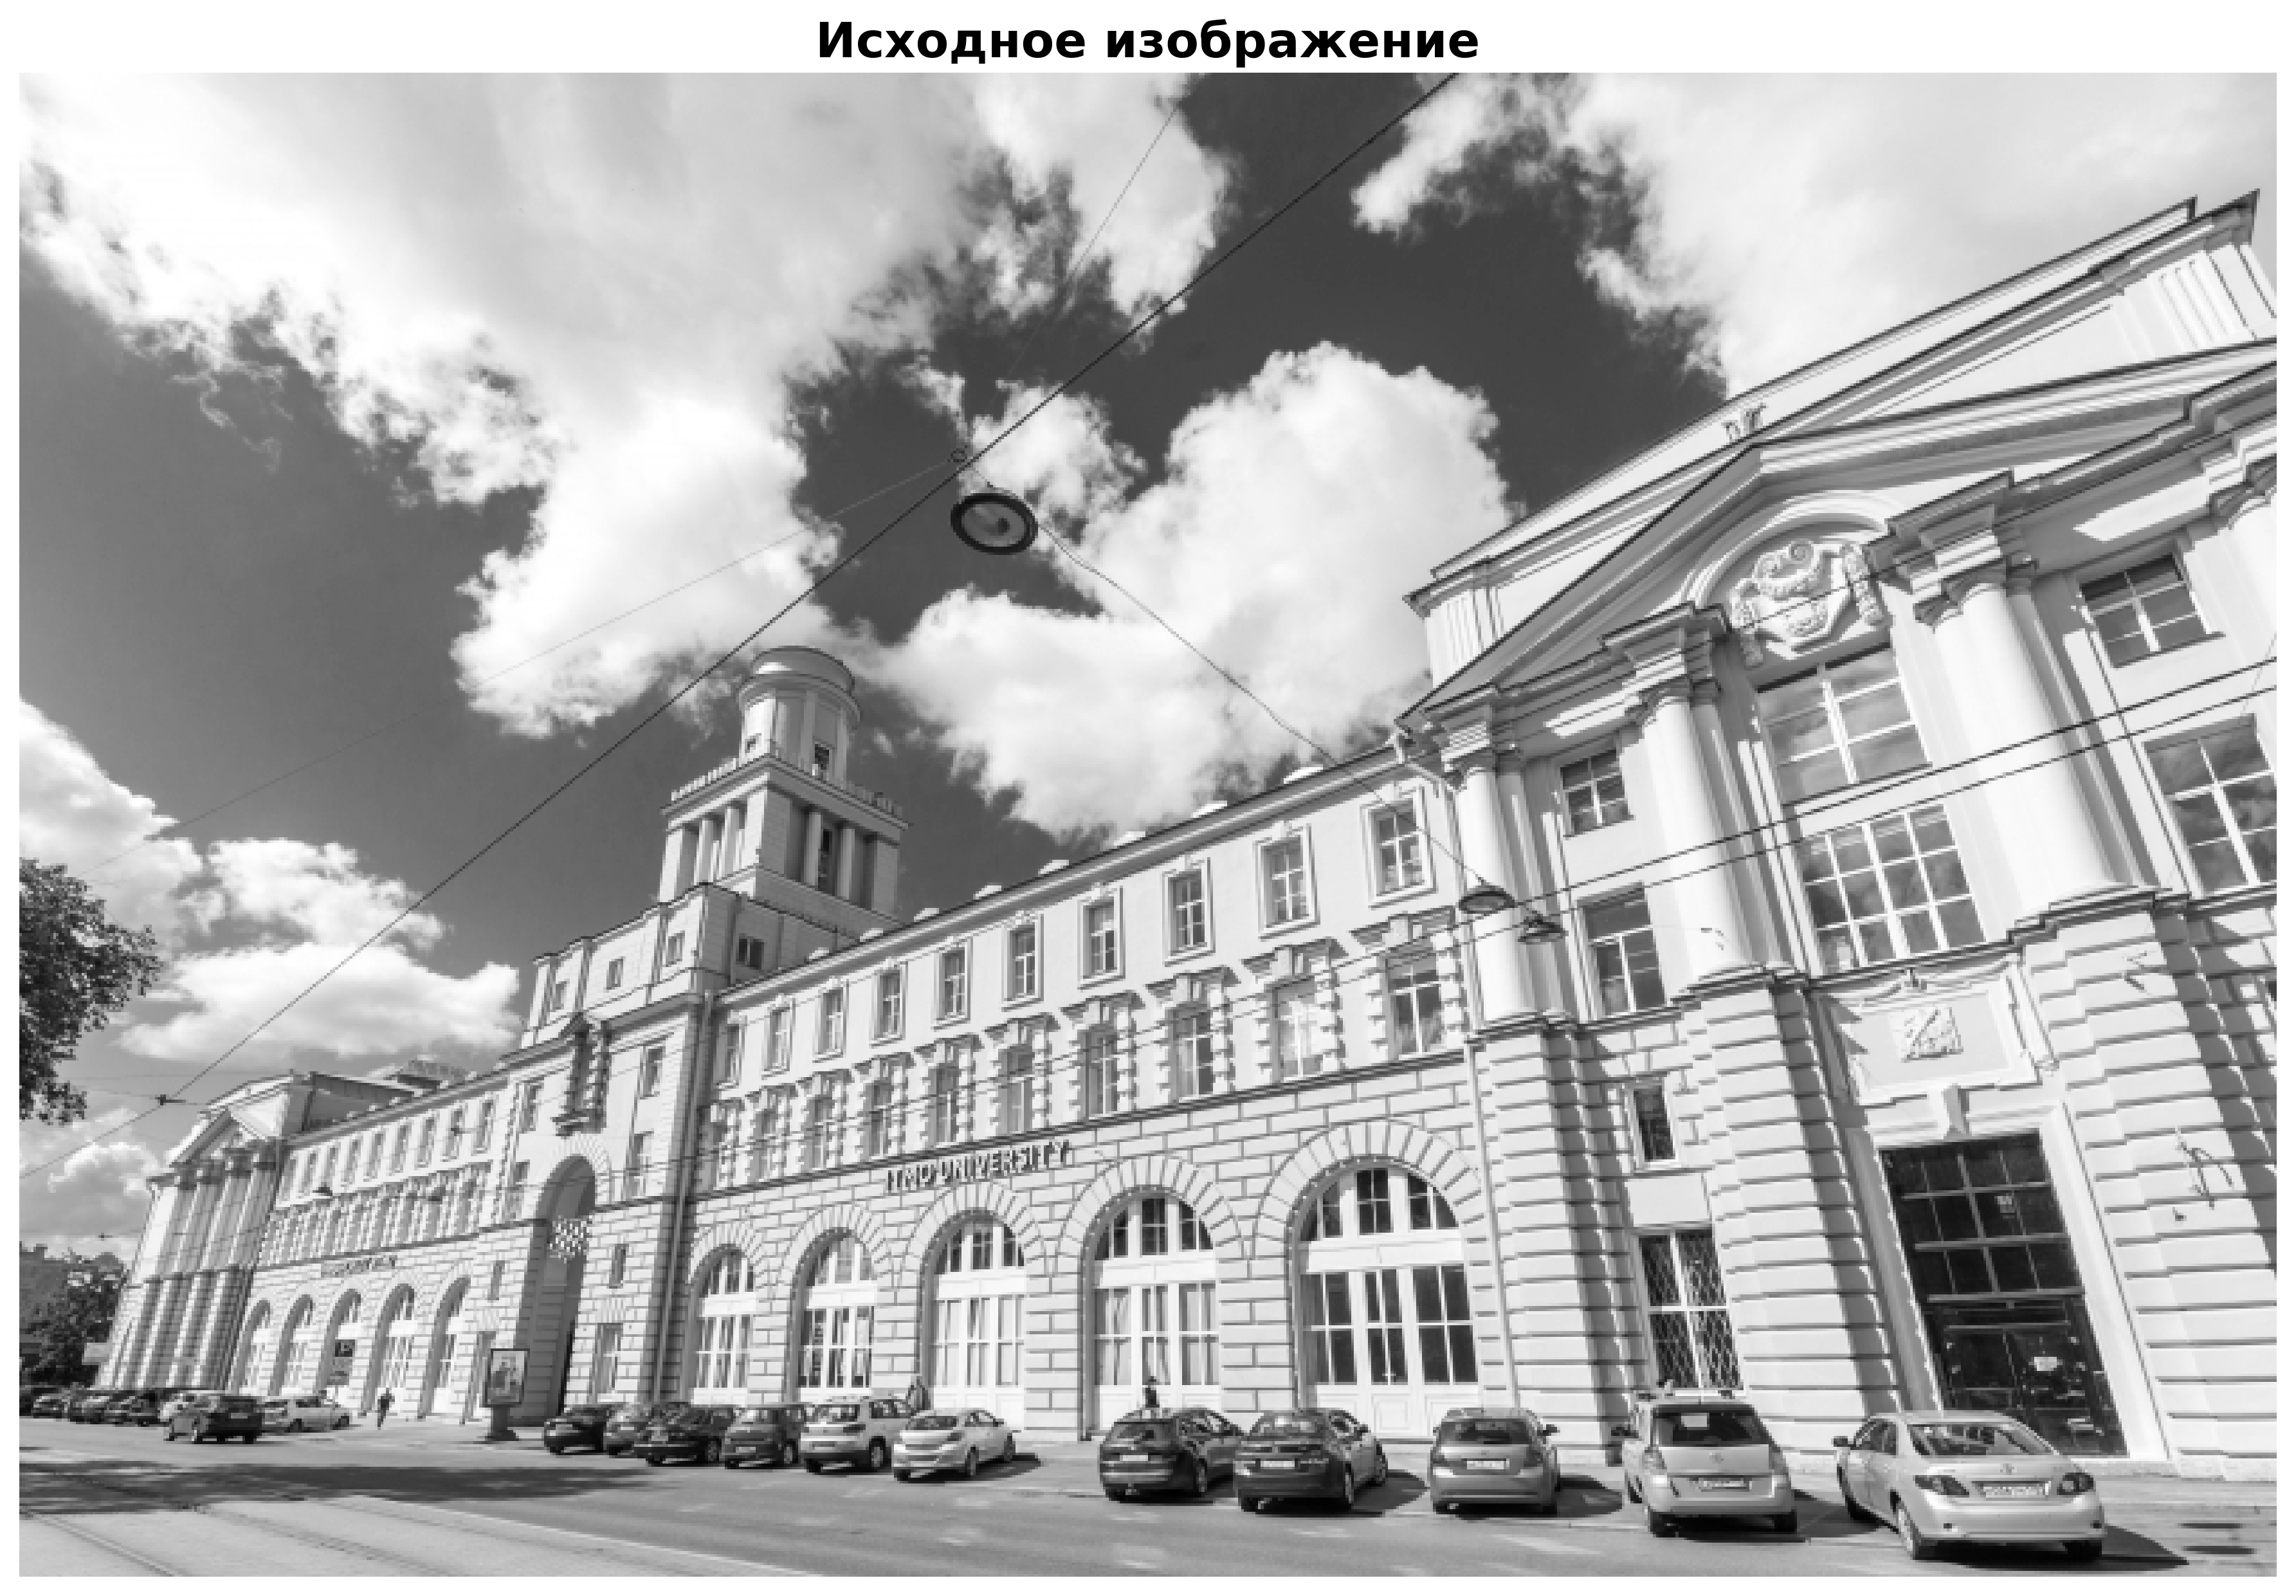
\includegraphics[width=0.6\linewidth]{images/task1/svd_original.png}
  \caption{Исходное изображение в оттенках серого}
  \label{fig:svd-original}
\end{figure}

\begin{figure}[h!]
  \centering
  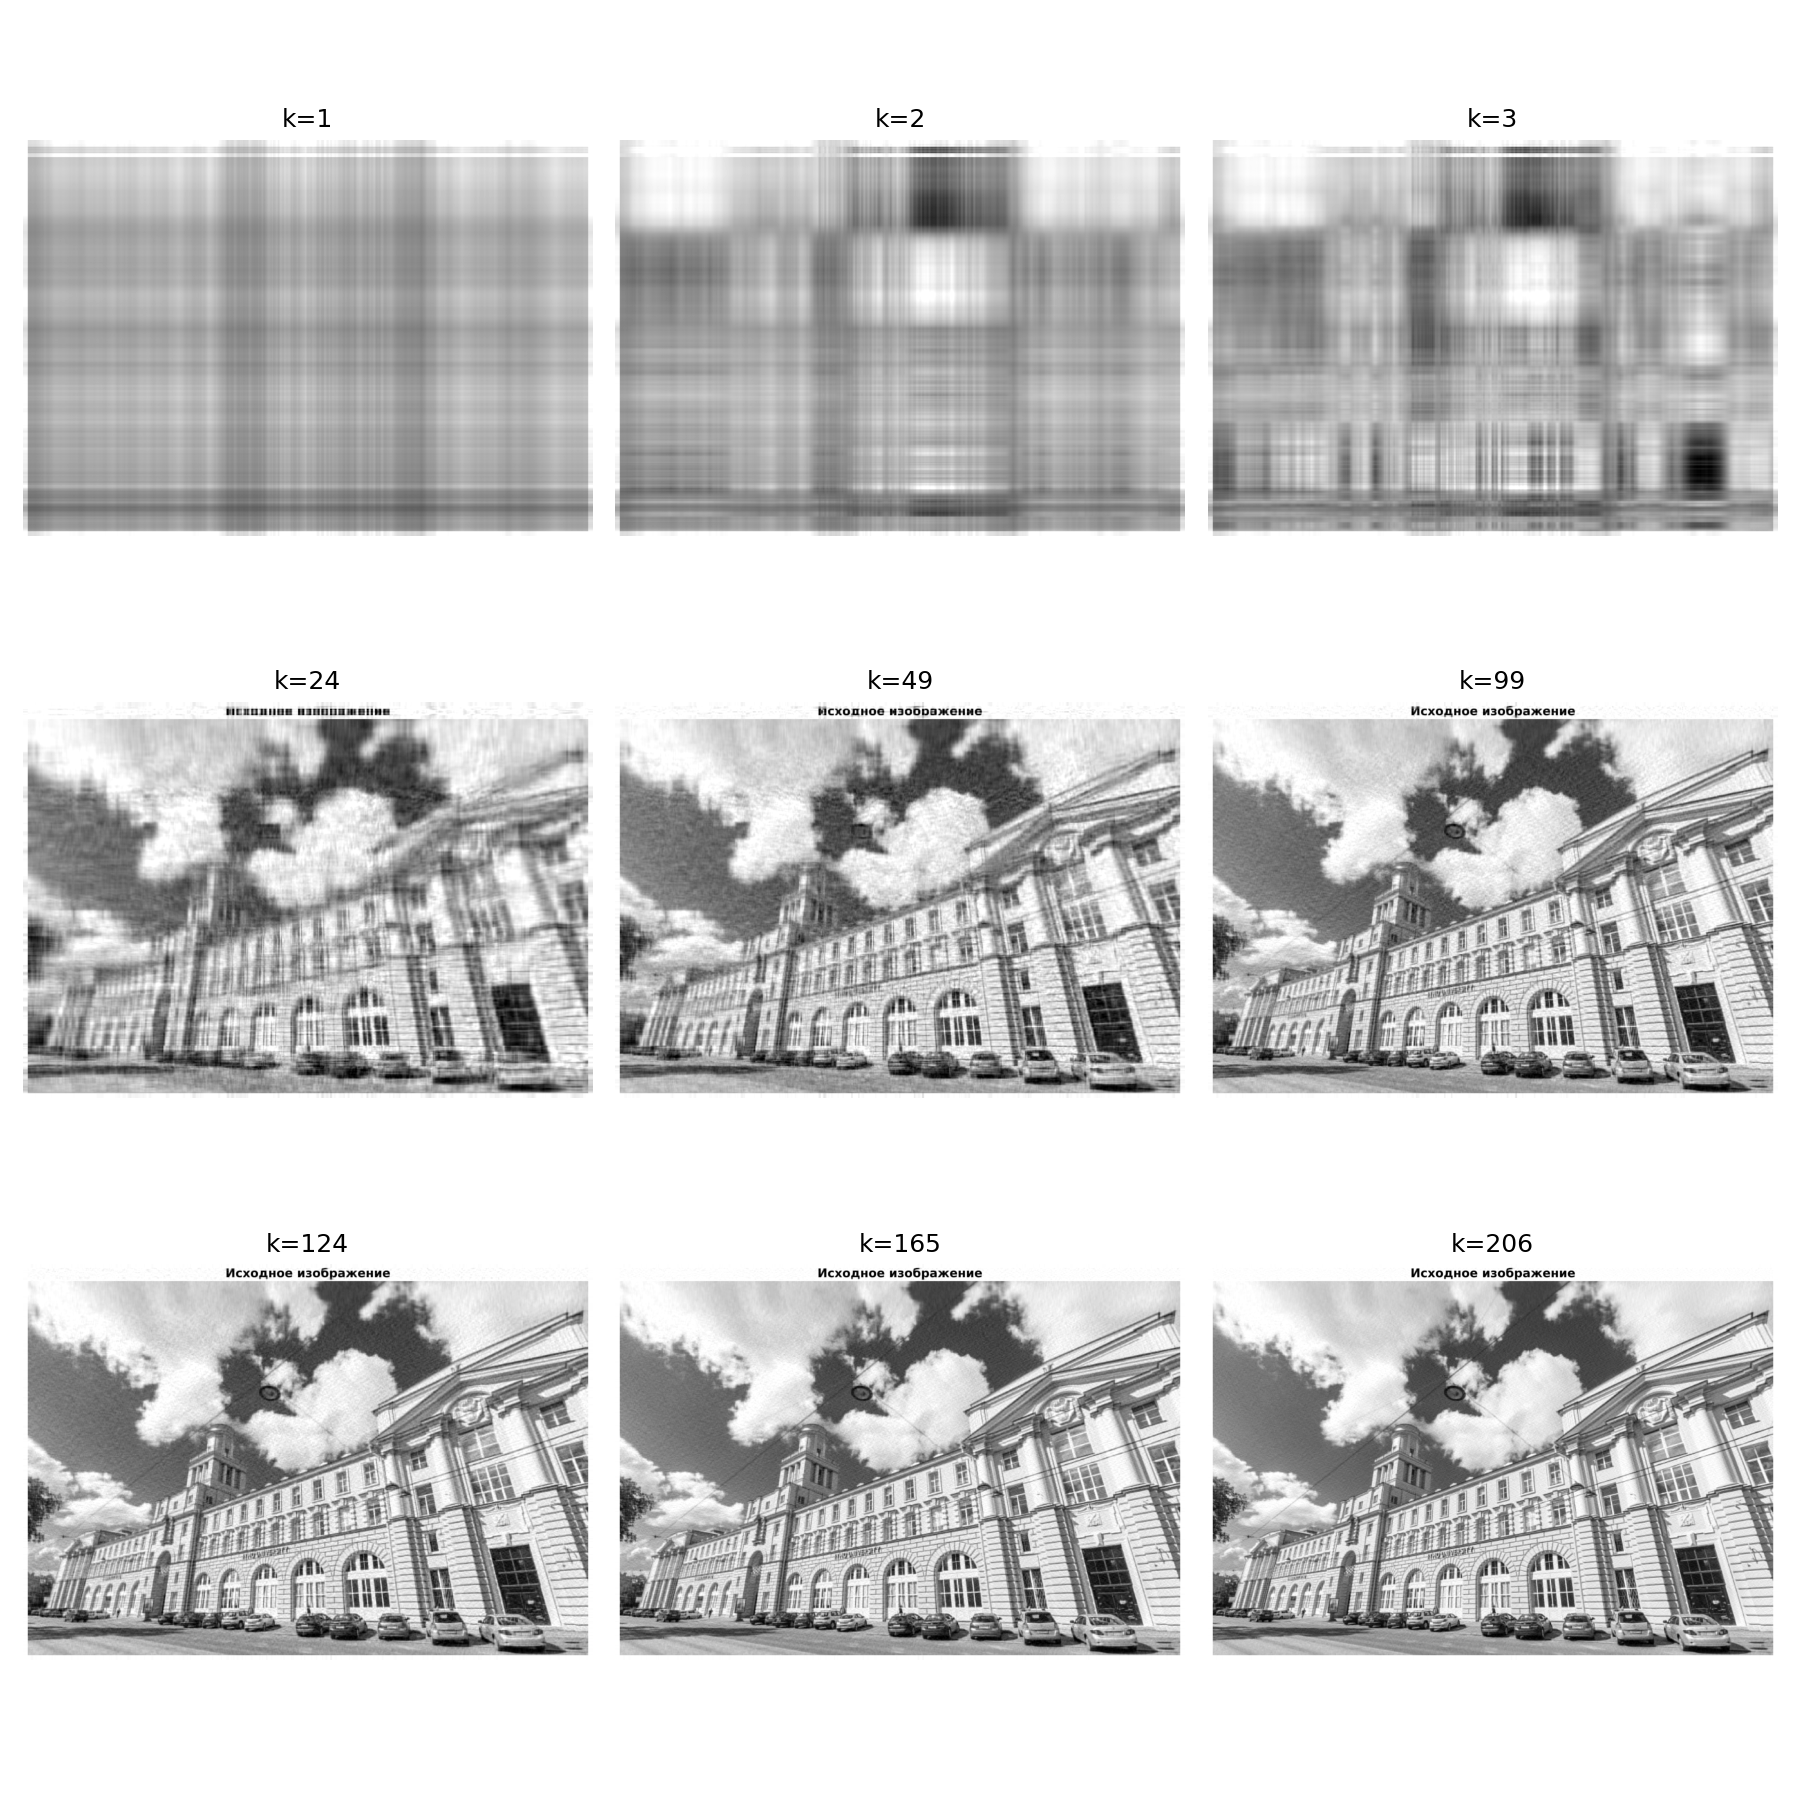
\includegraphics[width=0.95\linewidth]{images/task1/svd_grid.png}
  \caption{Реконструкции при различных \(k\) (9 вариантов)}
  \label{fig:svd-grid}
\end{figure}

\begin{figure}[h!]
  \centering
  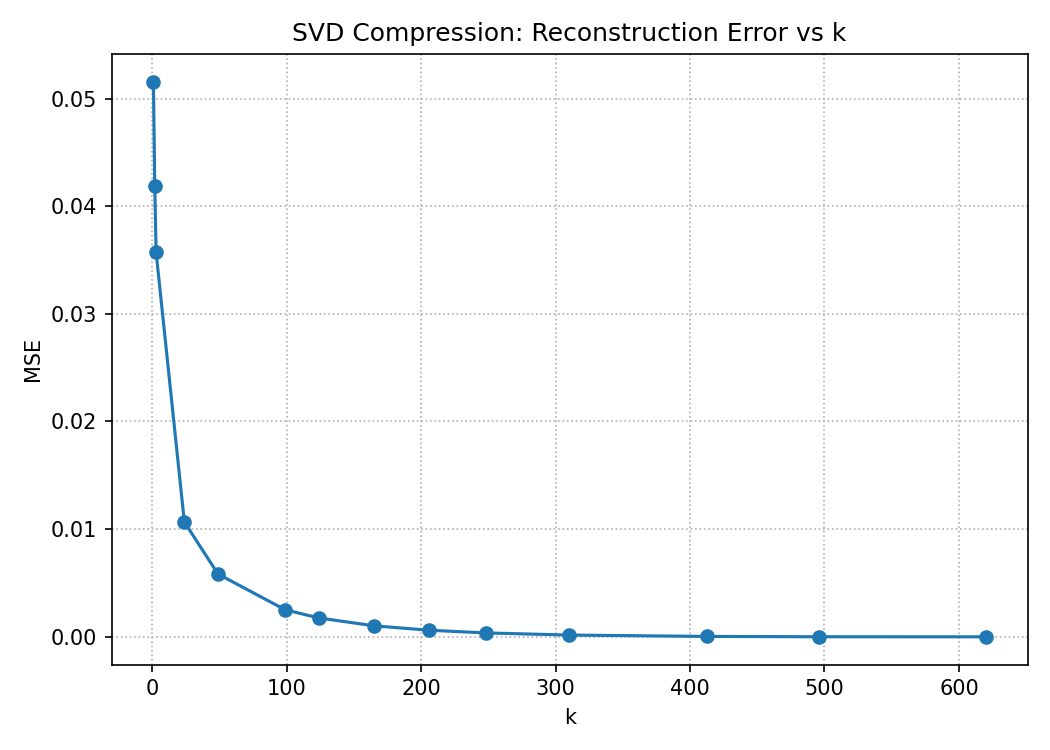
\includegraphics[width=0.48\linewidth]{images/task1/svd_mse_vs_k.png}\hfill
  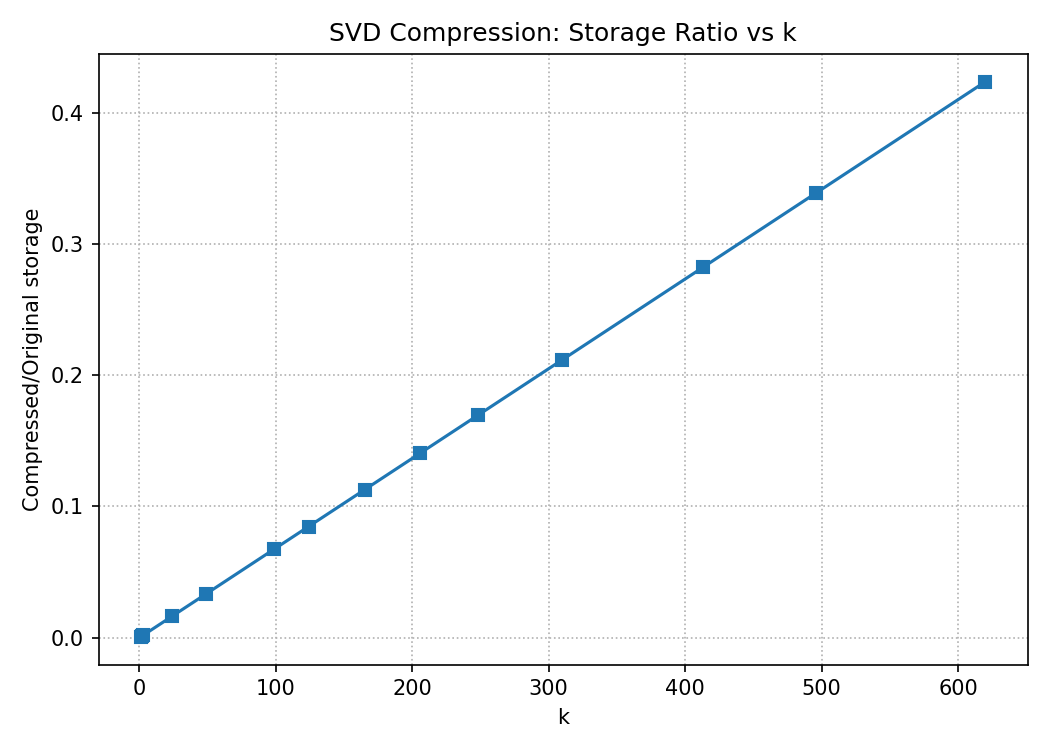
\includegraphics[width=0.48\linewidth]{images/task1/svd_storage_ratio_vs_k.png}
  \caption{Зависимость ошибки (MSE) и относительного объёма хранения от \(k\)}
  \label{fig:svd-metrics}
\end{figure}

\subsection*{Анализ результатов}
\begin{itemize}
  \item При малых \(k\) (\(1\)–\(3\)) картинка сильно теряет детали и становится расплывчатой; она уже распознаваема, но качество невысокое.
  \item При средних \(k\) видны основные контуры и крупные детали; качество приемлемое при заметном снижении объёма хранения.
  \item При больших \(k\) визуально близко к исходному, но выигрыш по памяти меньше.
\end{itemize}

\section*{Задание 2. Latent Semantic Analysis (LSA)}

Для набора текстовых документов был выполнен предобработчик: удаление пунктуации и цифр, приведение к нижнему регистру, токенизация, лемматизация (\texttt{pymorphy2}) и исключение стоп-слов (встроенный список). По очищенной коллекции построена терм-документная матрица (TF–IDF-подобное взвешивание), затем выполнено SVD-разложение.

В качестве корпуса использован файл \texttt{PLA/lab6/python/data12.txt} (22 коротких документа).

Ниже приведены: спектр сингулярных чисел, а также визуализации двух тем — топ-5 слов в каждой теме и облака слов.

Дополнительно построено «облако слов» по всему корпусу (без разбиения на темы).

\begin{figure}[h!]
  \centering
  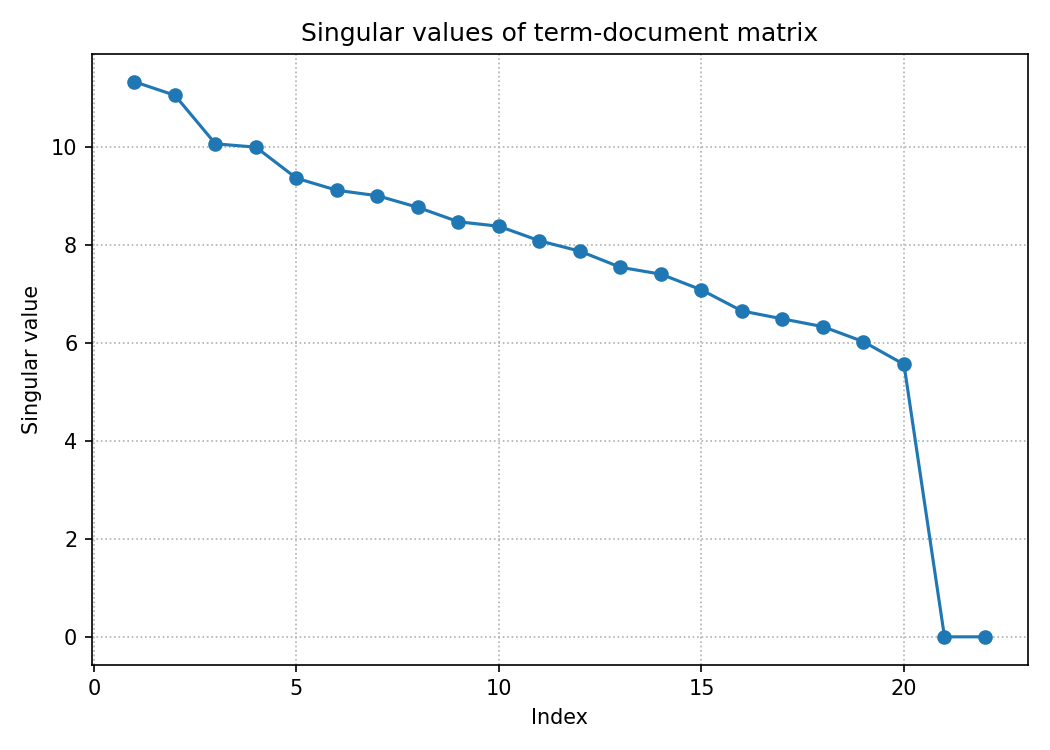
\includegraphics[width=0.6\linewidth]{images/task2/singular_values.png}
  \caption{Сингулярные числа терм-документной матрицы}
  \label{fig:lsa-svals}
\end{figure}

\begin{figure}[h!]
  \centering
  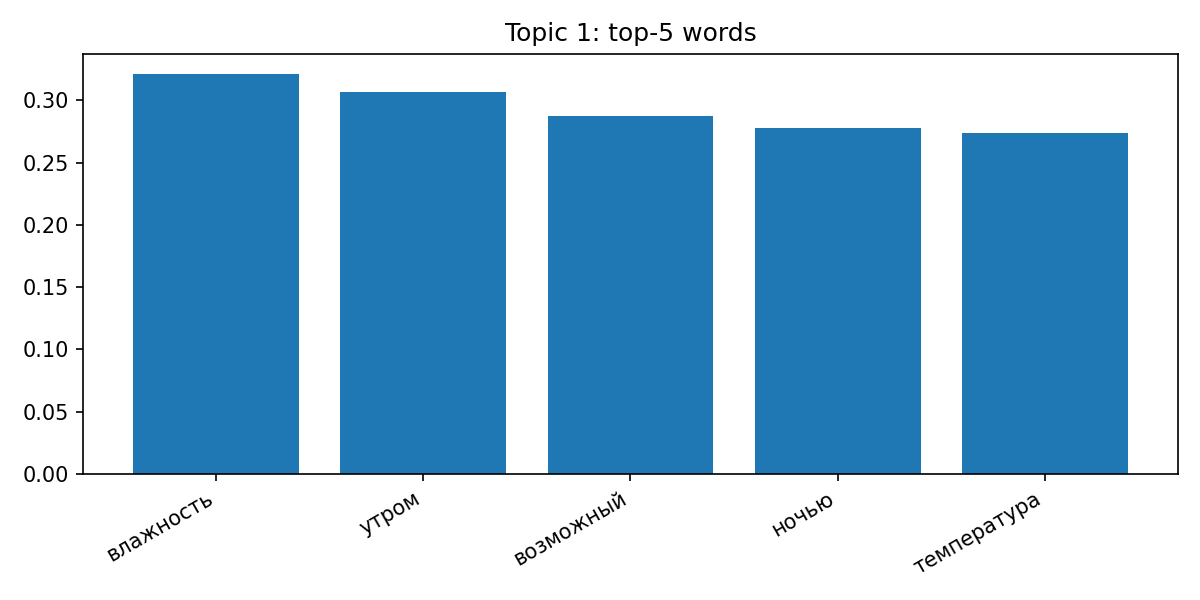
\includegraphics[width=0.48\linewidth]{images/task2/topic1_top_words.png}\hfill
  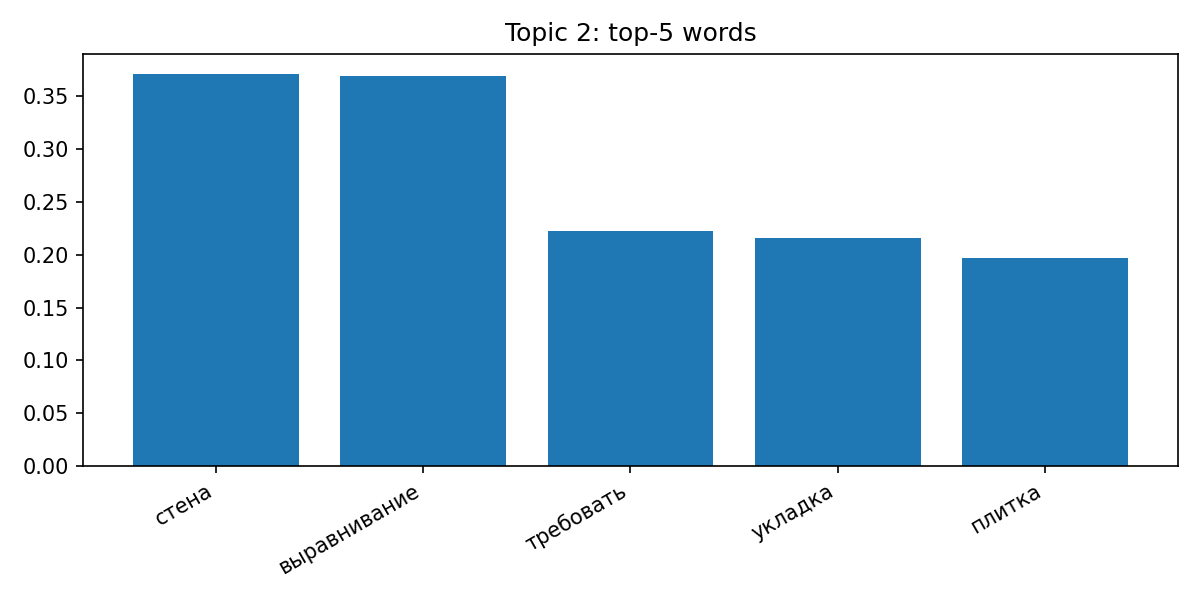
\includegraphics[width=0.48\linewidth]{images/task2/topic2_top_words.png}
  \caption{Топ-5 слов по абсолютному вкладу в двух ведущих темах}
  \label{fig:lsa-topwords}
\end{figure}

\begin{figure}[h!]
  \centering
  
\includegraphics[width=0.48\linewidth]{images/task2/topic1_wordcloud.png}\hfill
  
\includegraphics[width=0.48\linewidth]{images/task2/topic2_wordcloud.png}
  \caption{Облака слов для двух тем}
  \label{fig:lsa-wordcloud}
\end{figure}

\begin{figure}[h!]
  \centering
  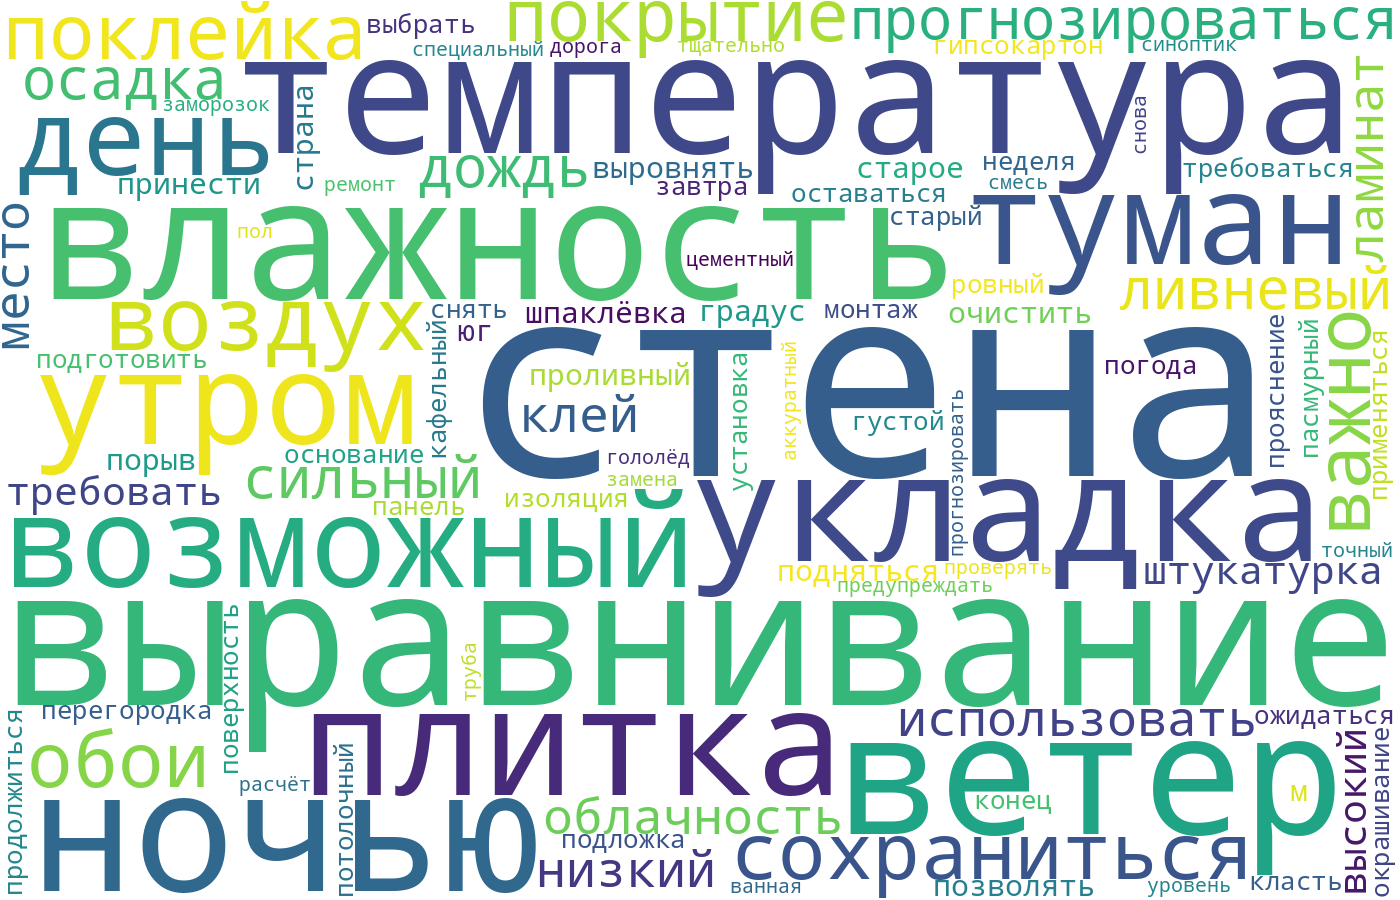
\includegraphics[width=0.7\linewidth]{images/task2/global_wordcloud.png}
  \caption{Глобальное облако слов по всему корпусу}
  \label{fig:lsa-global-wordcloud}
\end{figure}

\subsection*{Краткий анализ}
Первая и вторая сингулярные компоненты отражают две главные латентные темы в коллекции. Слова с наибольшими по модулю весами в соответствующих векторах \(U\) формируют смысловое ядро тем; компоненты вектора \(V\) позволяют определить документы, максимально связанные с каждой темой.

Для использованного примера (см. рис.~\ref{fig:lsa-topwords},~\ref{fig:lsa-wordcloud}) темы интерпретируются так: Тема 1 — метео/прогноз погоды (\emph{влажност, утр, температур, ноч, возможн}); сильнее всего связаны документы Doc~20, Doc~2, Doc~16, Doc~12, Doc~8. Тема 2 — ремонт/отделка (\emph{стен, выравниван, треб, укладк, плитк}); сильнее всего связаны документы Doc~19, Doc~15, Doc~21, Doc~7, Doc~3.

\section*{Выводы по проделанной работе}
\begin{itemize}
  \item По задаче SVD-сжатия: при малых \(k\) изображение заметно теряет детали; при средних \(k\) качество уже приемлемое при разумном уменьшении объёма хранения; при больших \(k\) картинка близка к исходной, но выигрыш по памяти снижается. Характерная зависимость MSE и доли хранения от \(k\) подтверждает ожидаемый компромисс «качество–сжатие».
  \item По задаче LSA: базовая предобработка (\texttt{pymorphy2}+стоп-слова) и SVD выделили две устойчивые темы — погода/прогноз и ремонт/отделка; связанные документы определяются по весам правых сингулярных векторов. Убывание сингулярных чисел указывает на низкоранговую структуру.
\end{itemize}

\section*{Приложение}
\subsection*{Текстовый корпус для LSA}
\begin{enumerate}
  \item Днём температура воздуха поднимется до +20 градусов, а ночью сохранится влажность.
  \item Перед поклейкой обоев важно очистить стены от старого покрытия.
  \item На юге страны прогнозируются сильные ветры и проливные дожди.
  \item Шпаклёвка позволяет выровнять стены перед поклейкой обоев.
  \item Ветер с порывами до 20 м/с принесёт ливневые осадки и облачность.
  \item Для укладки плитки требуется подготовить поверхность и выбрать клей.
  \item Температура остаётся низкой, прогнозируются осадки и облачность.
  \item Гипсокартон используют для выравнивания стен и монтажа перегородок.
  \item Пасмурная погода сохранится, местами возможен сильный ветер.
  \item Укладка ламината требует ровного основания и подложки для изоляции.
  \item Завтра утром ожидается густой туман и высокая влажность.
  \item Перед установкой потолочных панелей важно снять старую штукатурку.
  \item Ливневые дожди продолжатся до конца недели, местами будет туман.
  \item Штукатурка применяется для выравнивания стен перед окрашиванием или укладкой плитки.
  \item Температура воздуха утром будет низкой, а днём возможны прояснения.
  \item Кафельную плитку кладут на специальный клей, тщательно проверяя уровень.
  \item Синоптики предупреждают о тумане и гололёде на дорогах ночью.
  \item Замена труб в ванной требует точного расчёта и аккуратного выравнивания стен.
  \item Ночью возможны заморозки, а утром снова прогнозируют высокую влажность.
  \item Для ремонта пола используют цементную смесь для выравнивания и покрытия ламинатом.
\end{enumerate}

